Before every training, the data must be carefully inspected and in most cases preselected and modified in order to efficiently train a neural network and avoid training issues such as overfitting and divergence.
To address these problems, we first have to split our data into two different sets, the \textit{training set} and \textit{test set}. If we were to use all of our data for training, there would not be a way to estimate whether our predictions are overfitted or not, because the model has already seen all of the data in training. To solve this, it is common to take about ten percent of the dataset as test set without showing it to the neural network during training. If our model is overfitting the training data, meaning only adapting to individual features in the images but not certain features that define the mass of galaxy clusters, the predictions on the test set will be worse than the predictions on the training set. This way we can easily spot any overfitting problems. An even more efficient way to spot overfitting is by also using a \textit{validation set}. This is similar to the test set in that it is not used for training the neural network. The difference to the test set however is, that it is used during training to evaluate the model's performance, meaning we can see how our predictions perform on an unseen dataset. It is possible though not ideal to use the test set as validation set. The only downside of this method is, that if we optimize our network during training by changing parameters in order to increase validation set accuracy, we can run into overfitting again if we don't use separate test and validation sets. In my training I will use $90\%$ of the dataset as training set and the remaining $10\%$ as test set and validation set because I won't change parameters during training. The galaxy clusters are randomly selected for each set to avoid any bias in differing sets. However, to compare model accuracy, the same training and test sets are being used in every training. Otherwise it is possible to have easier or harder test sets for the model to evaluate which makes a comparison difficult.

\begin{table*}[h]
\centering
\begin{tabular}{@{}lr@{}}\toprule
\textbf{Dataset} & \textbf{Entries} \\
\midrule
Complete Set & $7946$ \\
Training Set & $7151$ \\
Test/Validation Set & $795$ \\
\bottomrule
\end{tabular}
\caption{Number of entries for the complete-, training-, test- and validation set of galaxy clusters.}
\label{tab:freq_bands}
\end{table*}

Ready-made models sometimes need a certain input format for training. ResNet for instance needs at least 71x71 pixels of image input to train. Moreover, it is not possible to provide it with more than three frequencies because it was developed to train with color images consisting of three channels, red, green and blue (RGB). To be able to train anyways, some changes to our dataset are needed. Firstly, a padding of 21x21 pixels is added to the images. With this we achieve the desired image size of 71x71 pixels (see \autoref{fig:cluster_comp_padded}). For the sake of comparison, I also provided the basic network with only three frequencies despite it being able to train on all ten (as used in \citet{Krippendorf_2023}). Next, we have to select three of our ten frequency bands to train with. I decided to use the frequency range ($455\text{eV} < \nu < 1070\text{eV}$) because it allowed to see features for both smaller and bigger galaxy clusters. 


\begin{figure}[H]
\centering
\begin{subfigure}{.4\textwidth}
  \centering
  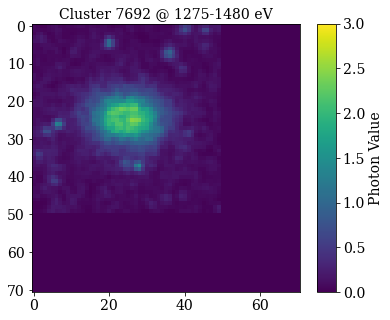
\includegraphics[width=\linewidth]{images/Chapter3/cluster_big_padded.png}
  \label{fig:cluster_big_padded}
\end{subfigure}%
\hspace{3.6em}
\begin{subfigure}{.4\textwidth}
  \centering
  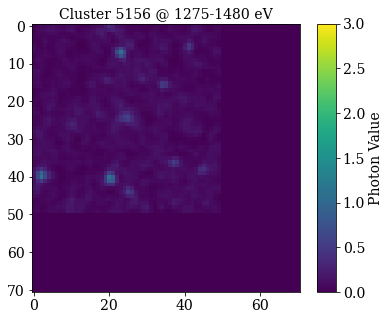
\includegraphics[width=\linewidth]{images/Chapter3/cluster_small_padded.png}
  \label{fig:cluster_small_padded}
\end{subfigure}
\caption{Galaxy clusters from \autoref{fig:cluster_comp} with the added padding of 21x21 pixels for training with deep models.} 
\label{fig:cluster_comp_padded}
\end{figure}

The final step before training is another randomization of our data. This helps to avoid any bias that our dataset already includes. There could be for example a bias in the way the simulation generates galaxy clusters, preferring a certain rotation. Because there is no designated direction in space, we expect galaxy clusters to be randomly rotated. Because of that, a random flip of each galaxy cluster image is performed before training.
This gives us the full data preparation pipeline as seen in \autoref{fig:pipeline}.

\begin{figure}[H]
\centering
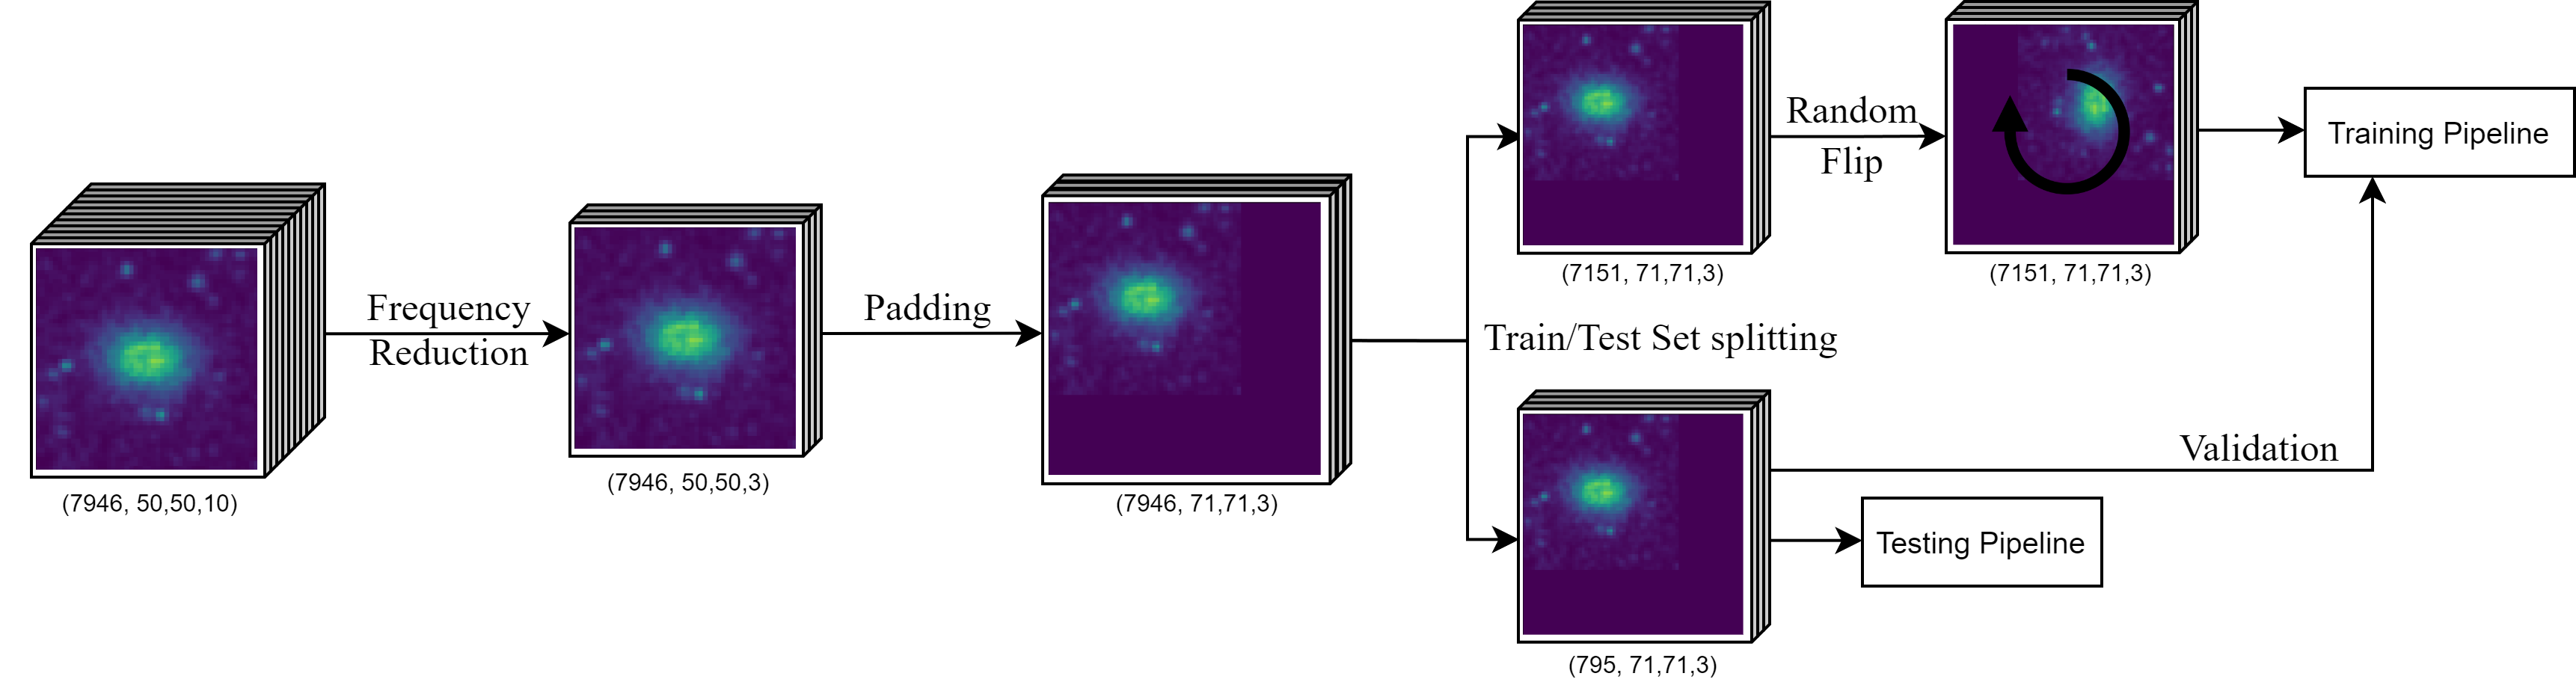
\includegraphics[width=\linewidth]{images/Chapter3/pipeline.png}
\caption{Full data preparation pipeline. The numbers below each step stand for (samples,x-image size,y-image size,frequencies)} 
\label{fig:pipeline}
\end{figure}